\chapter{Combinations and interpretations of Run 1 searches for invisibly decaying Higgs bosons}
\label{chap:comb}
Whilst the \ac{VBF} production mode offers the best sensitivity to invisibly decaying Higgs bosons, the limits on \BRinv can be improved by taking into account searches performed using other production channels. According to the $CL_{S}$ method described in \SectionRef{sec:stats} multiple searches can be combined by constructing a likelihood, according to \EquationRef{eq:likelihood}, which takes into account the regions of all the analyses. Combinations of the \ac{VBF} analyses with the other channels are described in sections \ref{sec:combotherchannels} to \ref{sec:combparked}. As well as combining the results of the \ac{VBF} searches with other channels, it is also possible to interpret them as limits on other specific models. Interpretations of the \ac{VBF} search results in several \ac{DM} models are described in \SectionRef{sec:dminterp}.

%??CHECK PLOT AXIS LABEL SIZES AND THAT LEGEND TERMS ARE STANDARD OR IN TEXT

\section{Searches in other channels}
\label{sec:combotherchannels}
%??Refer back to theory to introduce ZH and ggH searches
As described in \SectionRef{sec:higprod} after \ac{VBF} the next most sensitive production modes to invisible Higgs boson decays are \ac{ggH} and \ac{VH}. \ac{VH} has a much lower rate than \ac{VBF} (approximately 4 times less for a 125 \GeV Higgs boson). Compensating for this low cross-section, several of the final states of \ac{VH} production, particularly \ac{ZH}, give very clean signatures which are easy to identify. \ac{ggH} has a much higher rate than \ac{VBF}, but in most cases the resulting Higgs boson is created alone. However, if there is \ac{ISR} this can result in one or more jets allowing this channel to also be used. 

Three invisibly decaying Higgs boson searches were carried out by CMS during Run 1 in addition to the \ac{VBF} analyses. Two of these searches specifically targeted the \ac{ZH} production mode, one searching for events where the \PZ boson decayed to two leptons (the \PZ$(\ell\ell)$H search) and one where it decayed to two b quarks (the \PZ$(b\bar{b})$H search). The third ``monojet'' search targets events with one or more jets that are not \ac{VBF}-like and includes categories targeting \ac{ggH} and \ac{VH} production where the vector boson decays hadronically. The fraction of the signal expected to come from each production mode in each category of each search along with the integrated luminosity used is given in \TableRef{tab:analysissummary}. The limits from each search alone on \BRinv for a 125 \GeV Higgs boson are given in \TableRef{tab:combinedlimits}.

%signal fraction table
\begin{table}
\caption{Summary of the analyses included in the combination. The first column is the name of the analysis. The second and third columns give the integrated luminosity of the 7 and 8 TeV data sets used by each analysis. The fourth column contains the names of the categories in each analysis and the fifth column gives the proportion of signal events expected to come from each Higgs boson production mode.}
           \begin{center}
           \begin{tabular}{lccc}
           \hline
           \multirow{2}{*}{Analysis} & Luminosity (\invfb) &\multirow{2}{*}{Category} & Expected signal \\
           \cline{2-2}
           & 8 TeV (7 TeV) & & composition \\
           \hline
           \hline
           VBF prompt data &  19.5 & 2-jet VBF & 94\% VBF, 6\% ggH \\
           \hline
           VBF parked data &  19.2 & 2-jet VBF & 92\% VBF, 8\% ggH \\
           \hline
           \multirow{6}{*}{Monojet} & \multirow{6}{*}{19.7} & Monojet & 70\% ggH, 20\% VBF, \\
            & & & 6\% WH, 3\% ZH \\
            & & unresolved & 47\% WH, 25\% ggH, \\
            & & &  23\% ZH, 5\% VBF \\
            & & resolved & 39\% ggH, 32\% WH, \\
            & & &  18\% ZH, 11\% VBF \\
           \hline
           \multirow{4}{*}{\PZ$(\ell\ell)$H} & \multirow{4}{*}{19.7 (4.9)} & \Pep\Pem - 0-jet & 100\% ZH \\
            & & \Pep\Pem - 1-jet &  100\% ZH\\
            & & \Pgmp\Pgmm - 0-jet &  100\% ZH\\
            & & \Pgmp\Pgmm - 1-jet &  100\% ZH\\
           \hline
           \multirow{3}{*}{\PZ$(b\bar{b})$H} & \multirow{3}{*}{18.9} & 2-b-jet - low \MET & 100\% ZH \\
            & & 2-b-jet - medium \MET &  100\% ZH\\
            & & 2-b-jet - high \MET &  100\% ZH\\
           \hline
           \end{tabular}
           \end{center}
           \label{tab:analysissummary}
\end{table}

%??individual limits
\begin{table}
\begin{center}
\caption{Summary of 95\% CL upper limits on $\frac{\sigma}{\sigma_{SM}}\cdot$\BRinv obtained from each individual search contributing to the combinations described in this section~\cite{Chatrchyan:2014tja,CMS-PAS-HIG-15-012}.}
        \begin{tabular}{lc}
                \hline
                \hline
                \multirow{2}{*}{Channel}        & Observed (expected) upper limits \\
                                                                                & on $\frac{\sigma}{\sigma_{SM}}\cdot$ \BRinv (\%)\\
                \hline
                \hline
                VBF prompt data               & 65 (49) \\
                VBF parked data               & 57 (40) \\
                \PZ$(\ell\ell)$H              & 84 (87) \\
                \PZ$(b\bar{b})$H              & 192 (198) \\ 
                Monojet                       & 54 (62) \\
                \hline
                \hline
        \end{tabular}
        \label{tab:combinedlimits}
\end{center}
\end{table}


When combining limits from separate analyses it is important that there is no overlap between the regions used by the analyses. A brief description of the event selection used in each of the non-\ac{VBF} invisibly decaying Higgs searches is therefore given in the following subsections. It is also important when constructing the overall likelihood function to understand which uncertainties are correlated between analyses and which are not. The uncertainties considered to be correlated between the analyses are discussed in Sections \ref{sec:combprompt} and \ref{sec:combparked}. 


\subsection{Z$(\ell\ell)$H$\rightarrow$invisible selection}
\label{sec:zllh}
%sel
The \PZ$(\ell\ell$)H search is described in Ref.~\cite{CMS-PAS-HIG-13-018}. The analysis selection requires two tight opposite charge same flavour leptons (either electrons or muons) both with \pt$>20$ \GeV, with invariant mass compatible with the \PZ boson, no further leptons and large \MET. Events containing two or more jets with \pt$>30$ \GeV are rejected to reduce the \PZ+jets background. 

To reduce backgrounds, in events with a single jet, that jet is required not to be identified using the \ac{CSV} algorithm (described in \SectionRef{sec:parkedtop}) as a b-jet. Also, requirements are made on the azimuthal angular separation and \pt balance between the \MET and the dilepton system. In addition to this signal region control regions, which differ from the signal region in that the lepton system is not compatible with a \PZ boson decay, are used for background estimation. Due to events with more than one jet being vetoed there is no overlap between the events in the signal or control regions of this analysis and the events selected in the \ac{VBF} and \PZ$(b\bar{b})$H analyses (where two jets with \pt$>30$ \GeV are required in all regions). 

\subsection{Z$(b\bar{b})$H$\rightarrow$invisible selection}
\label{sec:zbbh}
%sel
The \PZ$(b\bar{b})$H search is described in Ref.~\cite{CMS-PAS-HIG-13-028}. The analysis selection requires two jets tagged by the \ac{CSV} algorithm as originating from b-quarks, large \MET, and no reconstructed electrons or muons. The di-b-jet system is required to have high \pt, but low invariant mass (less than 250 \GeV). The dijet mass cut ensures there is no overlap with either of the \ac{VBF} analyses. The main background to the analysis is from \ac{QCD} multijet processes as in the \ac{VBF} analysis. Similarly to the selection of the parked data \ac{VBF} analysis this background is reduced using requirements on \jetmetdphi and \METsig. The neutral component of the \MET is also required to be aligned with the charged component in $\phi$. The signal region is separated into three categories with with low, medium and high \MET and control regions where the signal region selections are relaxed or inverted are used to estimate the remaining backgrounds.

\subsection{Monojet selection}
\label{sec:monojet}
%sel
The ``monojet'' search, is described in Ref.~\cite{CMS-PAS-EXO-12-055}. This analysis selects events with large \MET, one or more high-\pt jets and no reconstructed electrons or muons. To separate events due to \ac{ggH} production with \ac{ISR} from those due to \ac{VH} production where the vector boson decays hadronically, events are classified into three signal categories. The categorisation is sequential, i.e. if an event passes the requirements for the first category it is not considered for the second etc. 

The first category targets ``unresolved'' vector bosons where the high \pt of the vector boson causes its decay products to be very close together. These unresolved vector bosons are identified by searching for so-called ``fat'' jets with substructure with \pt$>200$ \GeV, (described in detail in Ref.~\cite{CMS-PAS-EXO-12-055}. One additional normal jet is allowed in this category as long as it is within 2 in $\phi$ of the fat jet.

The second category is the resolved category where the vector boson has lower \pt and its decay products can be identified as two separate normal jets. These jets are required to have an invariant mass between 60 and 110 \GeV, which overlaps with the range used in the \PZ$(b\bar{b})$H analysis regions, leading to a non-negligible overlap in the events selected. The resolved category is therefore not used in any combinations.

The third category is the ``monojet'' category. Events in this category are required to have one jet with \pt$>150$ \GeV. One additional jet within 2 in $\phi$ of the first jet is allowed to be present, with further jets causing the event to be vetoed. Control regions, which differ from the above categories by the presence of one or more leptons or photons, are used to perform background estimations. Finally, the category definitions above are not orthogonal to the \ac{VBF} analysis. To remedy this any events passing the \ac{VBF} parked data analysis selection were vetoed. This veto removes less than 4\% of the expected signal events in the monojet category and none of the signal events expected in the resolved category. As the monojet analysis was performed in 2015, after the parked data \ac{VBF} analysis had been performed, the monojet analysis was not combined with the prompt analysis. Therefore, no overlap veto between these two analyses was necessary.

The lepton veto present in all three signal categories means there is no overlap of any of the three categories with the \PZ$(\ell\ell)$H analysis regions. Some of the control regions do overlap slightly with regions of the \PZ$(\ell\ell)$H search, however these overlaps are very small due to the very high jet \pt cut present in the monojet search. In addition to the \PZ$(b\bar{b})$H search overlapping with the resolved category, there are also overlaps between the \PZ$(b\bar{b})$H search and the  unresolved and monojet categories. However, very few events in the \PZ$(b\bar{b})$H search have jets with \pt$>150$ \GeV, so these overlaps are considered negligible.

\section{Combination with prompt data VBF search}
\label{sec:combprompt}
%Present combination
The first combination that was performed was between the analyses that were completed in 2013, the two \PZ$\rm{H}$ searches and the promt data \ac{VBF} search. As has been described above the regions used in these analyses do not overlap, however, as the objects used are very similar all three analyses several of the systematic uncertainties are correlated. The full list of correlated uncertainties, and the analyses they affect are given in decreasing order of the change in the expected limit on \BRinv for a 125 \GeV Higgs boson as a result of removing the uncertainty in \TableRef{tab:promptcorrs}. The method for determining jet energy in the \PZ$(b\bar{b})$H analysis, involving a regression technique~\cite{CMS-PAS-HIG-13-028}, is very different from that used in the other two analyses. The jet uncertainties are therefore correlated between the \PZ$(\ell\ell)$H and \ac{VBF} searches, but not the \PZ$(b\bar{b})$H analysis.

%correlation decisions
\begin{table}
  \caption{Uncertainties correlated between the \ac{VBF} prompt data, \PZ$(\ell\ell)$H and \PZ$(b\bar{b})$H searches and the analyses they affect. Also quoted is the relative change in the expected limit on \BRinv on removing each uncertainty from the analysis.}
  \label{tab:promptcorrs}
  \begin{tabular}{lcc}
    \hline
    \hline
    Uncertainty & Analyses affected & $\frac{\Delta(\rm(limit))}{\rm{limit}}$ on removal \\
    \hline
    \ac{JES} & VBF, Z($\ell\ell$)H & -0.13 \\
    PDFs & VBF, Z($b\bar{b}$), Z($\ell\ell$)H & -10 \\
    QCD scale & VBF, Z($b\bar{b}$), Z($\ell\ell$)H & -0.04\\
    Luminosity & VBF, Z($b\bar{b}$)H, Z($\ell\ell$)H & -0.02\\
    \ac{JER} & VBF, Z($\ell\ell$)H & $<$0.01\\
    Unclustered energy scale & VBF, Z($b\bar{b}$)H, Z($\ell\ell$)H & $<$0.01\\
    Lepton efficiency & VBF, Z($\ell\ell$)H & $<$0.01\\
    \hline
    \hline
  \end{tabular}
\end{table}

%interpolation
None of the analyses saw any significant excess of events, so limits were set using the asymptotic $CL_{S}$ procedure described in \SectionRef{sec:stats}. The Higgs boson mass hypotheses which the three analyses have generated \ac{MC} samples for are not the same. Between 115 and 145 \GeV the two \PZ$\rm{H}$ analyses have samples for the same masses. Limits from the combination of these two analyses were therefore obtained in this range and can be seen in \FigureRef{fig:zhcomb}. Assuming \ac{SM} Higgs boson production and acceptance the 95\% \ac{CL} observed (expected) limit on \BRinv is found to be 0.81 (0.83).

To combine the \PZ$\rm{H}$ and \ac{VBF} analyses it was necessary to interpolate the efficiency for the \ac{VBF} analysis to select \ac{VBF} and \ac{ggH} signal events between the available mass points (these ranged from 110 to 400 \GeV). Multiplying these interpolated efficiencies by the Higgs boson production cross-sections at a given mass allows a signal yield estimate for the \ac{VBF} analysis at that mass to be obtained. In order to combine limits from multiple production channels it is also necessary to make an assumption about the relative cross-section of these two production mechanisms. Assuming the \ac{SM} production cross-sections a combination was performed between all three analyses in the mass range 115 to 145 \GeV. The results of this combination can be seen in \FigureRef{fig:promptcomb}. The 95\% \ac{CL} observed (expected) limit on \BRinv was found to be 0.58 (0.44). The \PZ$(b\bar{b})$H search has no \ac{MC} samples available for Higgs boson masses above 145 \GeV, but the \PZ$(\ell\ell)$H search has samples up to 300 \GeV. The \ac{VBF} and \PZ$(\ell\ell)$H searches were therefore combined in the mass range 115 to 300 \GeV. The results of this combination can be seen in \FigureRef{fig:promptcombhighmass}.

\begin{figure}
  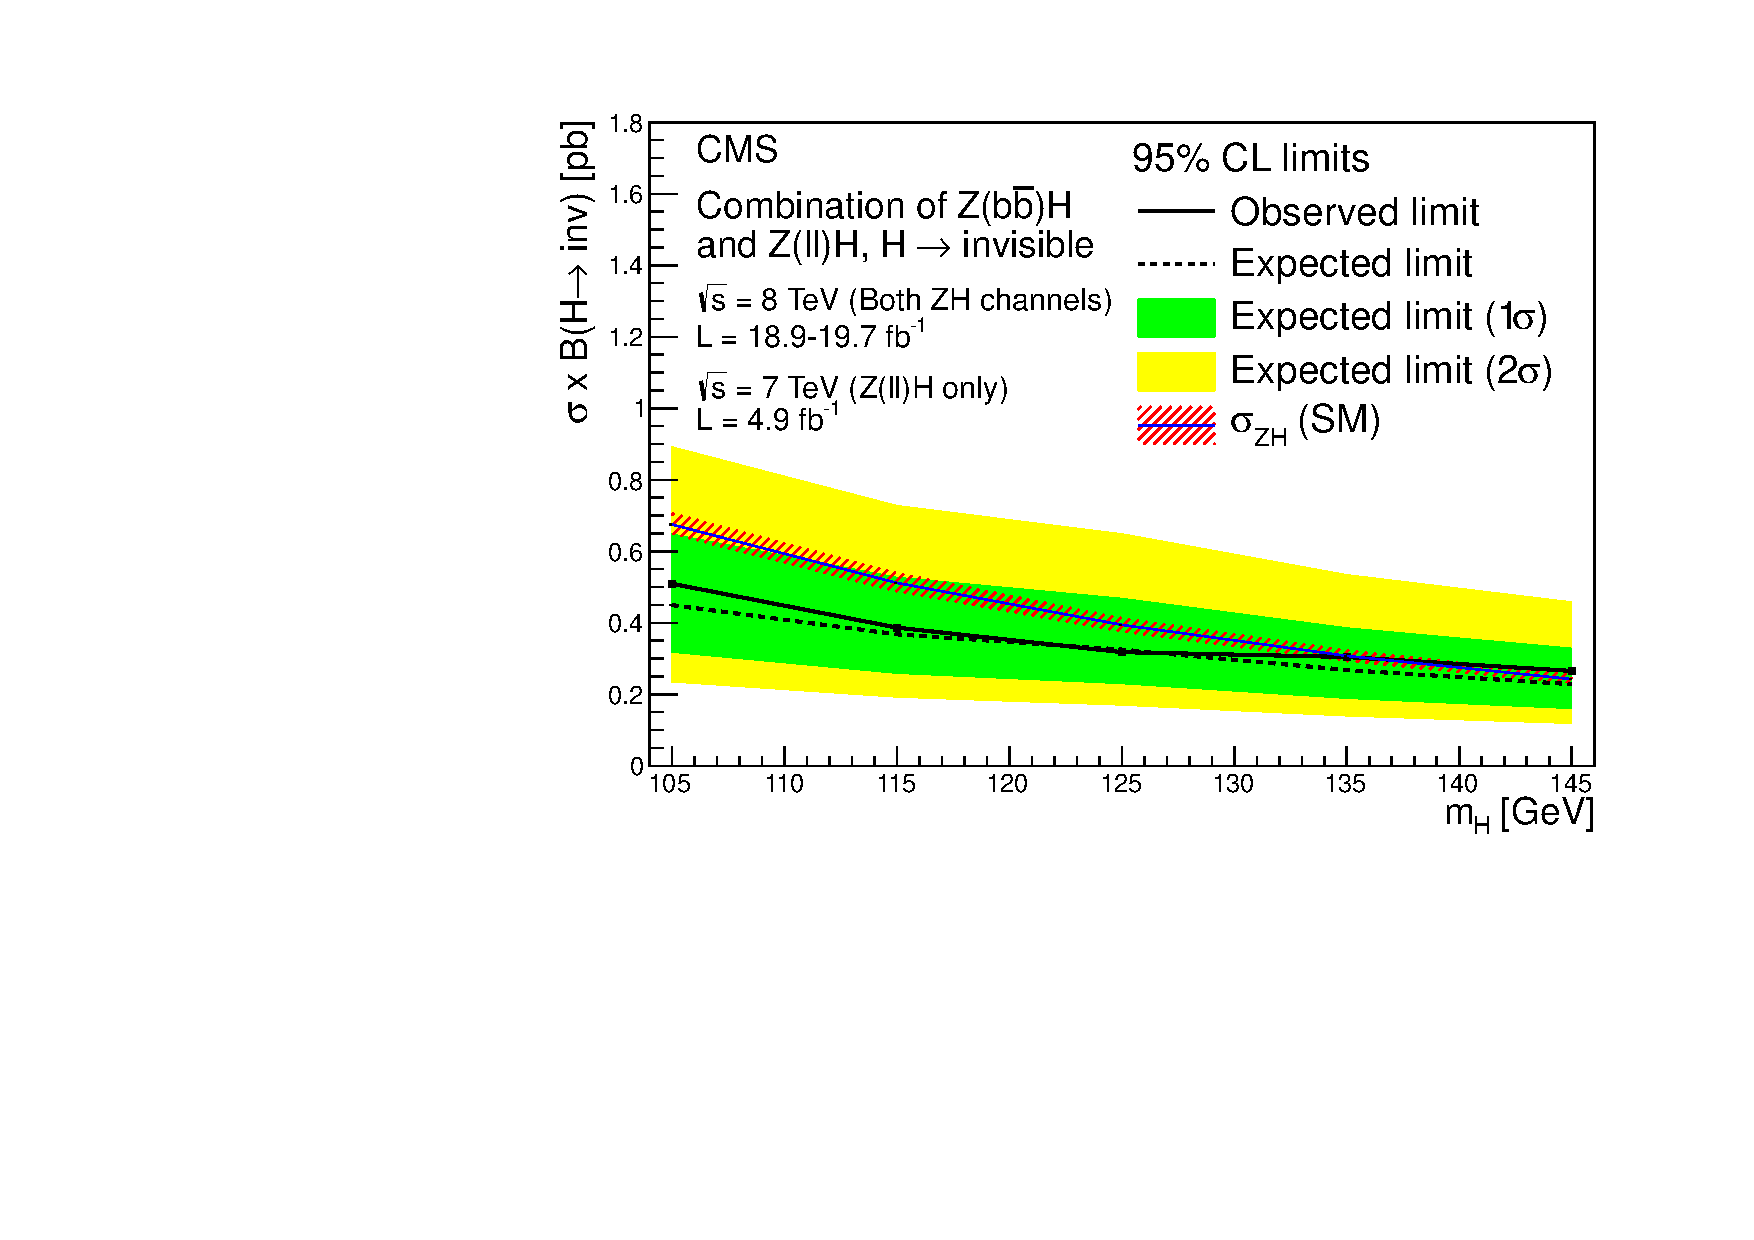
\includegraphics[width=.65\largefigwidth]{plots/prompt/HIG-13-30-figs/zhxslimit.pdf}
  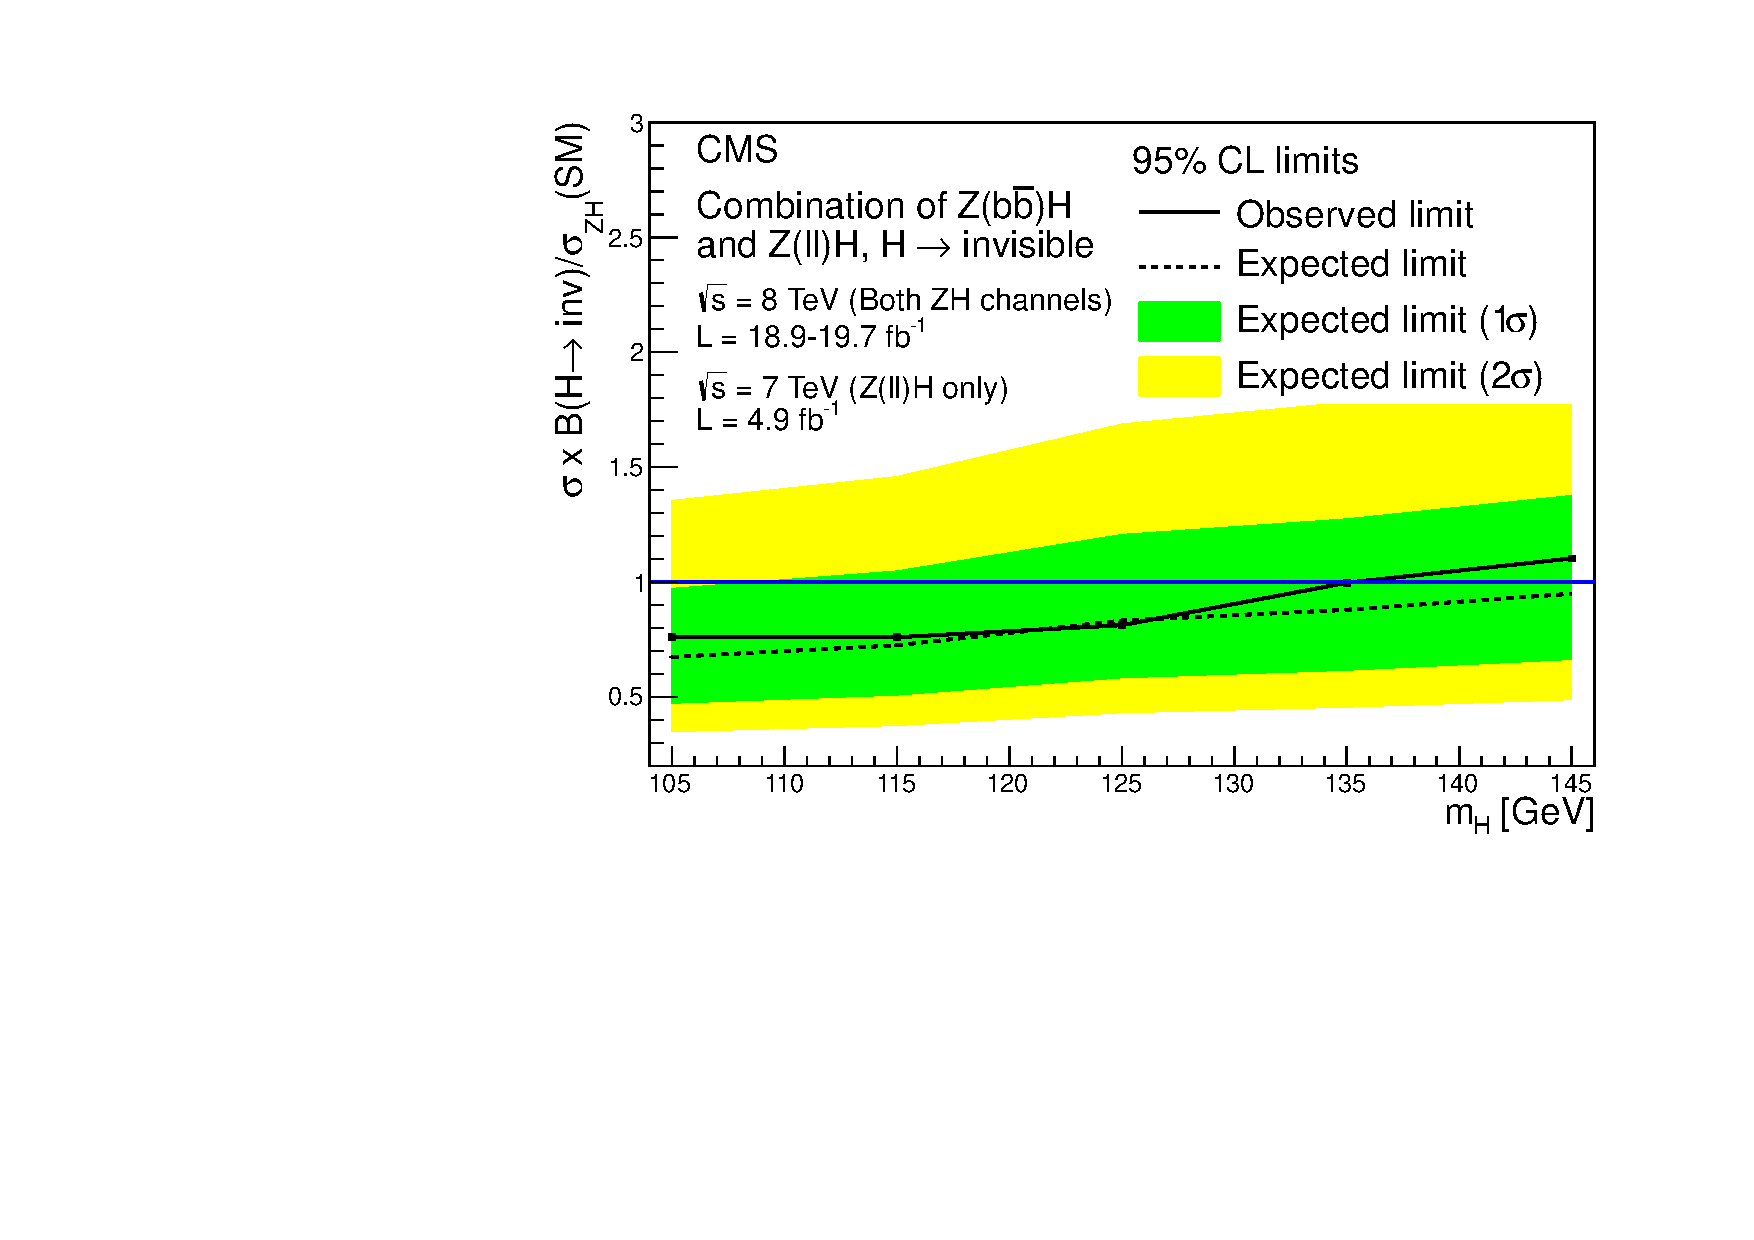
\includegraphics[width=.65\largefigwidth]{plots/prompt/HIG-13-30-figs/zhlimit.pdf}
  \caption{Expected and observed 95\% \ac{CL} upper limits on the \ac{ZH} $\sigma\times\mathcal{B}$ in \pb (a) and normalised to the SM \ac{VBF} Higgs boson production cross-section (b) obtained from the combination of the \PZ$(\ell\ell)$H and \PZ$(b\bar{b})$H searches~\cite{Chatrchyan:2014tja}. The green and yellow bands are the one and two sigma uncertainty bands of the expected limit~\cite{Chatrchyan:2014tja}.}
  \label{fig:zhcomb}
\end{figure}

\begin{figure}
  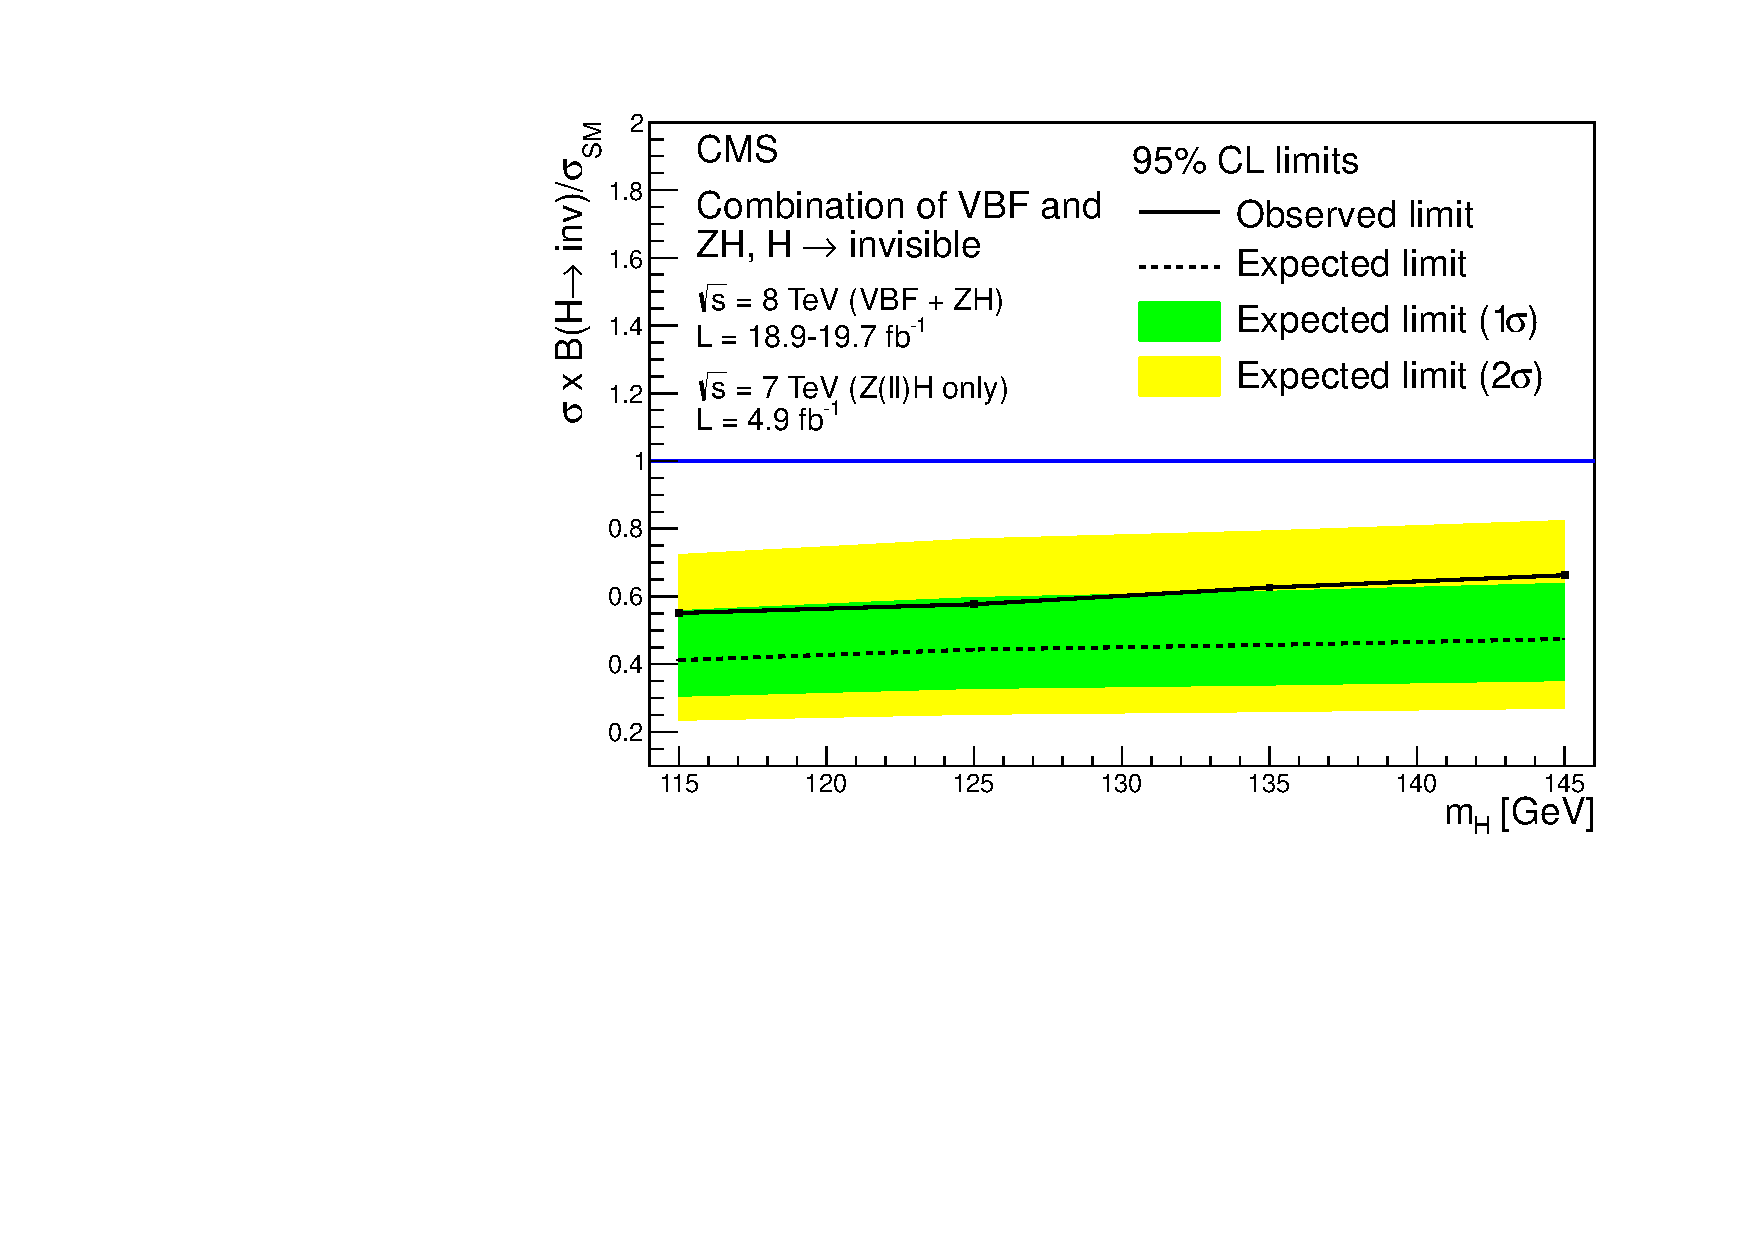
\includegraphics[width=\largefigwidth]{plots/prompt/HIG-13-30-figs/combinedlimit.pdf}
  \caption{Expected and observed 95\% \ac{CL} upper limits on the $\sigma\times\mathcal{B}/\sigma_{SM}$ obtained from the combination of the \ac{VBF}, \PZ$(\ell\ell)$H and \PZ$(b\bar{b})$H searches~\cite{Chatrchyan:2014tja}. The green and yellow bands are the one and two sigma uncertainty bands of the expected limit~\cite{Chatrchyan:2014tja}.}
  \label{fig:promptcomb}
\end{figure}

\begin{figure}
  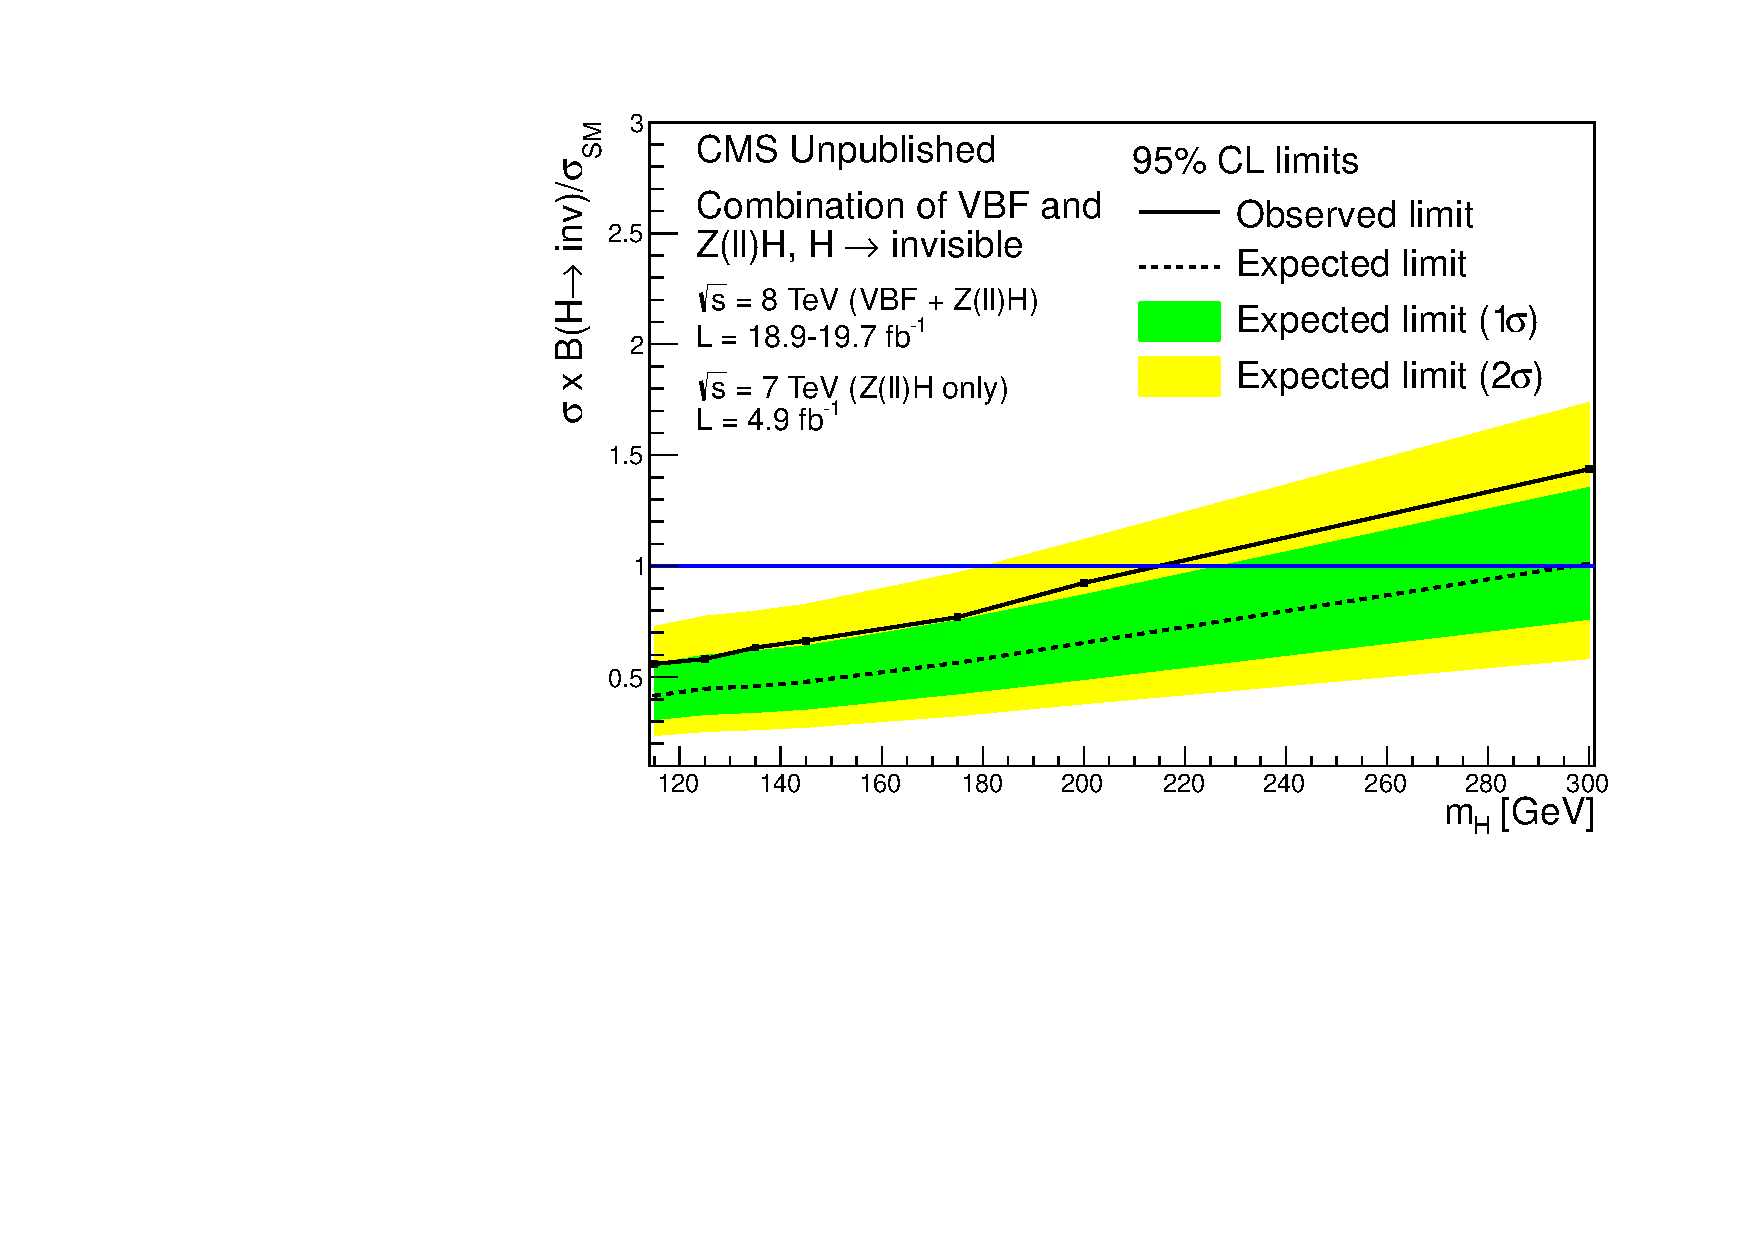
\includegraphics[width=\largefigwidth]{plots/prompt/HIG-13-30-figs/highmasslimit.pdf}
  \caption{Expected and observed 95\% \ac{CL} upper limits on the $\sigma\times\mathcal{B}/\sigma_{SM}$ obtained from the combination of the \ac{VBF} and \PZ$(\ell\ell)$H searches~\cite{Chatrchyan:2014tja}. The green and yellow bands are the one and two sigma uncertainty bands of the expected limit~\cite{Chatrchyan:2014tja}.}
  \label{fig:promptcombhighmass}
\end{figure}

\section{Combination with the parked data VBF search}
\label{sec:combparked}
%??Present combination
The parked data \ac{VBF} analysis was combined with both the \PZ$\rm{H}$ searches and the monojet search, which was finished in 2015~\cite{CMS-PAS-HIG-15-012}. The prompt data \ac{VBF} analysis was not included in this combination due to its large overlap with the parked data analysis. As dicussed above overlaps between the regions of the \ac{VBF} and monojet searches were explicitly removed by vetoing events in the monojet search passing the \ac{VBF} selection. The resolved category of the monojet search was also removed from the combination to avoid large overlap with the \PZ$(b\bar{b})$H search. This removal did not change the expected limit as the resolved category is the least sensitive to invisibly decaying Higgs bosons. The remaining overlaps between the monojet search and the \PZ$\rm{H}$ searches are small as discussed in \SectionRef{sec:monojet}.

%syst studies, correlation of JES,JER and why met scale in monojet not correlated why zbbH as above
After resolving the issue of overlaps it was necessary to study the correlations of systematic uncertainties between the searches. A summary of the correlated uncertainties, and the analyses they affect is given in \TableRef{tab:parkedcorrs}. Of particular note are the decisions taken in correlating the jet and \MET uncertainties. All 4 searches have an uncertainty due to \ac{JES} and \ac{JER}. As in the combination with the \ac{VBF} prompt data analysis the uncertainties on the jet energy in the \PZ($b\bar{b})$H analysis are not correlated with the other analyses due to the very different method of determining the jet energy. The \ac{JES} and \ac{JER} uncertainties vary as functions of a jets \pt and $\eta$, so it is important to study the jet kinematic distributions when deciding which of the remaining analyses should have correlated jet energy uncertainties. As described in \SectionRef{sec:monojet} the two categories of the monojet search used in this combination require very high \pt jets which are mostly in the central region of the detector. By contrast the \ac{VBF} parked data analysis' high \pt jets are mostly in the forward region of the detector due to the large \detajj requirement. The \PZ$(\ell\ell)$H analysis uses low \pt jets with \pt$>30$ \GeV similar to those used to calculate \jetmetdphi in the \ac{VBF} analysis, but very different from the monojet analysis high \pt central jets. The decision was therefore taken to correlate the \ac{VBF} and \PZ$(\ell\ell)$H analyses \ac{JES} and \ac{JER} uncertainties and to leave those from the monojet analysis uncorrelated.

In the case of the \MET uncertainties, the two \PZ$\rm{H}$ searches and the \ac{VBF} search use the same \MET corrections, whereas the monojet search applies a different set of corrections~\cite{CMS-PAS-EXO-12-055}. The monojet analysis \ac{UES} uncertainty was therefore not correlated with that from the other analyses.

\begin{table}
  \caption{Uncertainties correlated between the \ac{VBF} parked data, \PZ$(\ell\ell)$H, \PZ$(b\bar{b})$H and monojet searches and the analyses they affect.}%??
  \label{tab:parkedcorrs}
  \begin{tabular}{|l|c|}
      \hline
      Nuisance & Analyses which it affects \\
      \hline
      \ac{JES} & VBF, Z($\ell\ell$)H \\
      PDFs & VBF, Z($b\bar{b}$), Z($\ell\ell$)H, monojet \\
      QCD scale & VBF, Z($b\bar{b}$), Z($\ell\ell$)H, monojet \\
      Luminosity & VBF, Z($b\bar{b}$)H, Z($\ell\ell$)H, monojet \\
      \ac{JER} & VBF, Z($\ell\ell$)H \\
      \ac{UES} & VBF, Z($b\bar{b}$)H, Z($\ell\ell$)H \\
      Muon identification efficiency & VBF, Z($\ell\ell$)H, monojet \\
      Electron identification efficiency & VBF, Z($\ell\ell$)H \\
      Diboson cross-section & VBF, monojet \\
      \hline
    \end{tabular}
\end{table}

%combination results and explain by channel
With these uncertainty correlations the four searches were combined for a Higgs boson mass of 125 \GeV assuming \ac{SM} production-cross sections for each channel. The 95\% \ac{CL} observed (expected) limit on \BRinv was found to be 0.36 (0.30). The log-likeilihood obtained as a function of \BRinv can be seen in \FigureRef{fig:parkedcombscan}.

\begin{figure}
  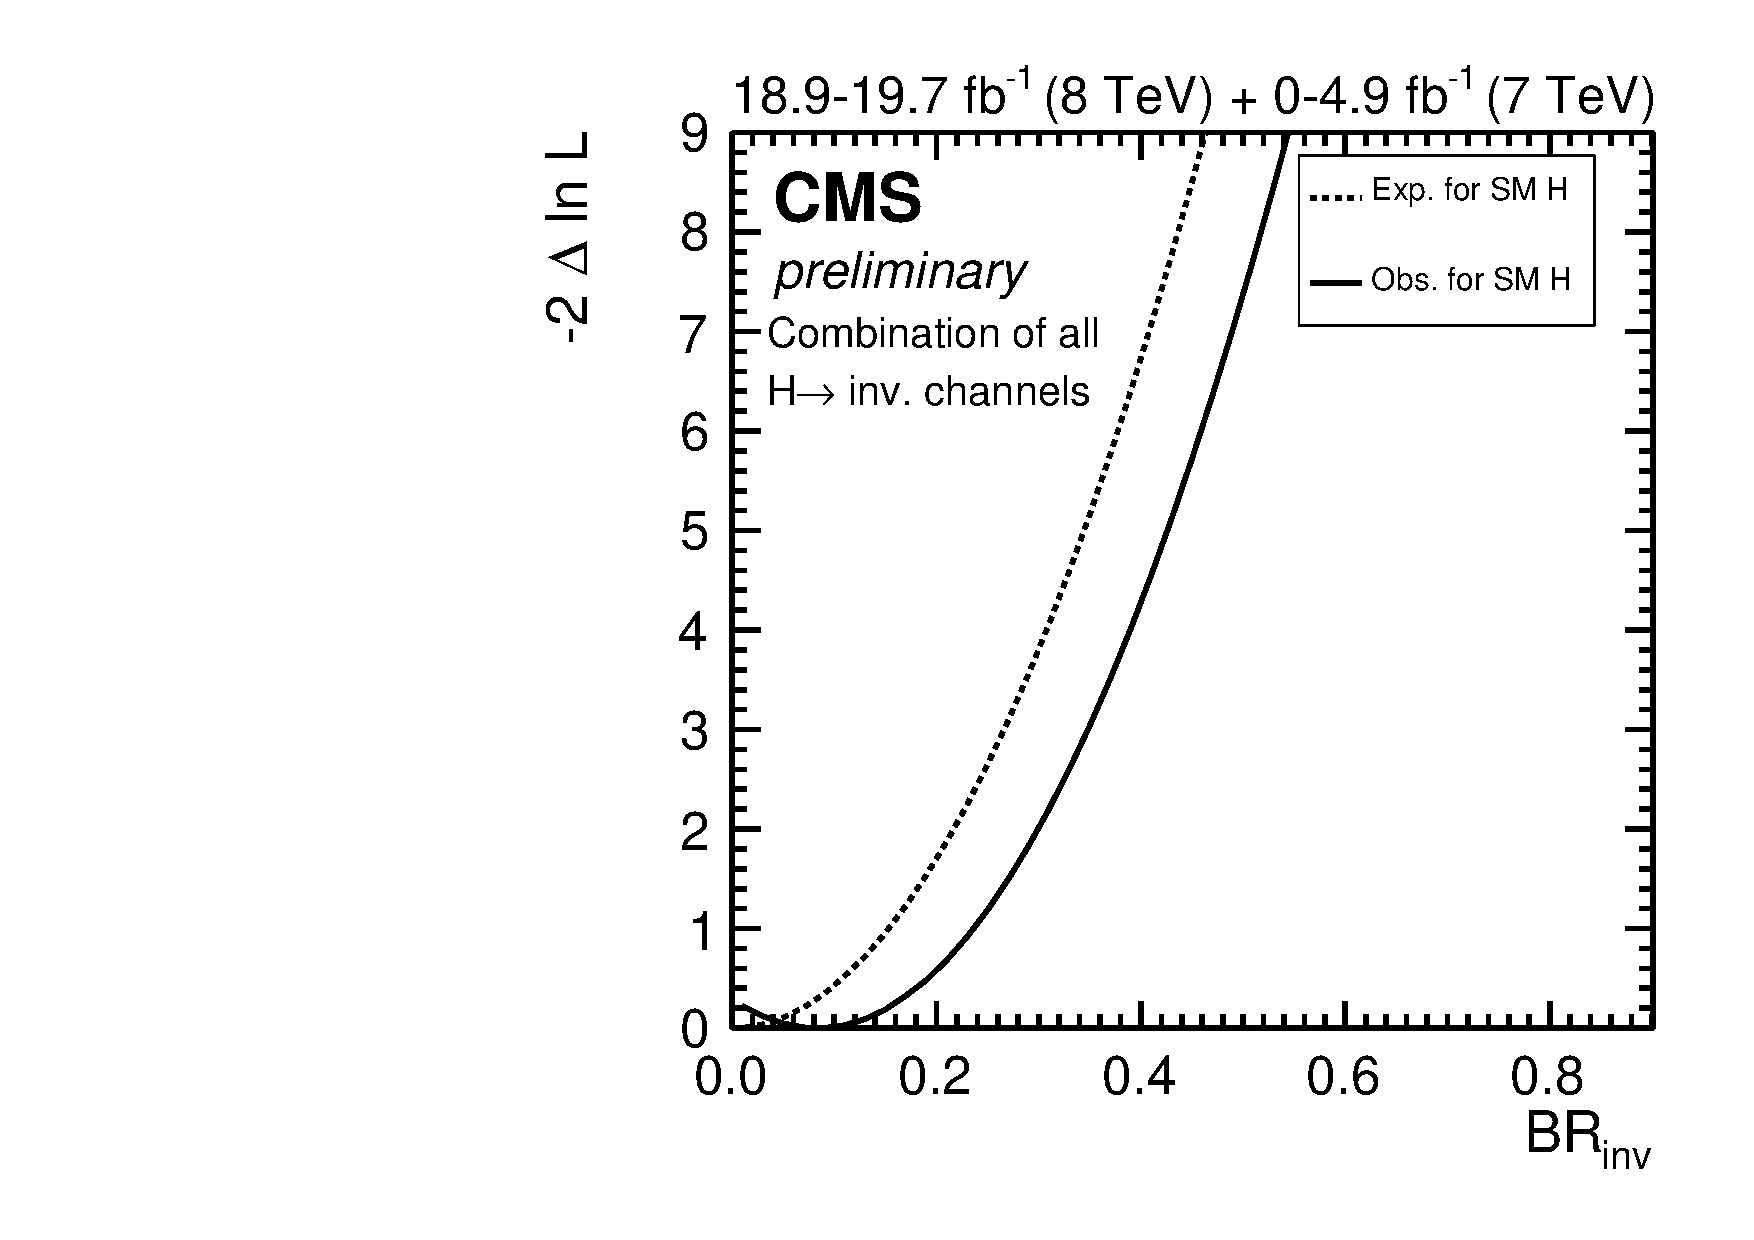
\includegraphics[width=\largefigwidth]{plots/comb/HIG-15-012-figs/combscan.pdf}
  \caption{Log-likelihood versus \BRinv. The solid curve represents the observation in data and the dashed curves represent the median expected result for no invisible decays of the Higgs boson~\cite{CMS-PAS-HIG-15-012}.}
  \label{fig:parkedcombscan}
\end{figure}

As well as the full combination of all analysis categories sub-combinations were also performed of all the categories targeting a particular production mode. The results of these sub-combinations and the full combination can be seen in \FigureRef{fig:parkedcombchannel}, where the \ac{VBF}-tagged limit comes from the \ac{VBF} parked data analysis, the \ac{VH}-tagged limit from the resolved category of the monojet analysis and the two \PZ$\rm{H}$ searches, and the \ac{ggH} tagged limit comes from the monojet category of the monojet analysis.

\begin{figure}
  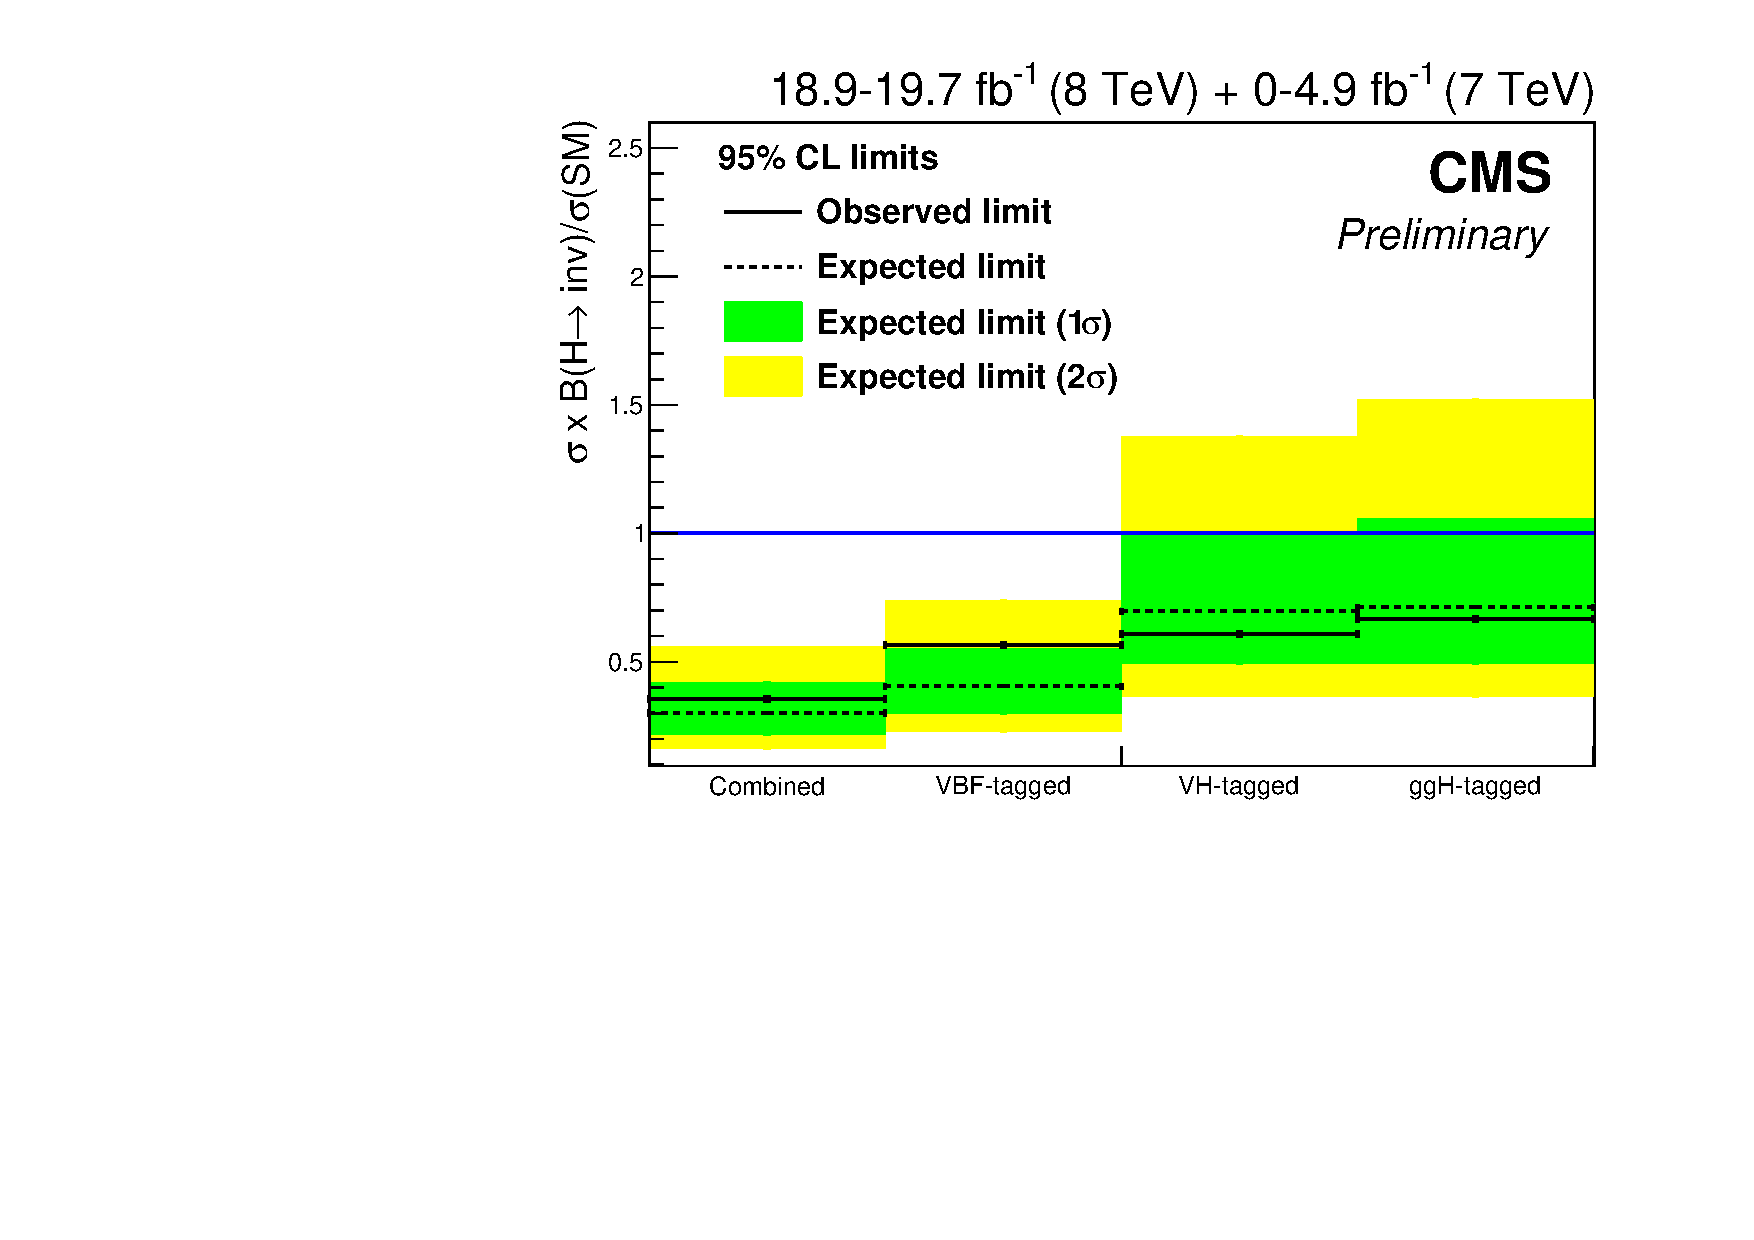
\includegraphics[width=\largefigwidth]{plots/comb/HIG-15-012-figs/channellimit.pdf}
  \caption{Expected and observed 95\% \ac{CL} upper limits on production cross section times \BRinv normalised tothe \ac{CM} production cross-section obtained from the combination of all channels targeting each Higgs boson production mode. The green and yellow bands indicate the 68\% and 95\% confidance intervals on the expected limit respectively~\cite{CMS-PAS-HIG-15-012}.}
  \label{fig:parkedcombchannel}
\end{figure}




\section{Dark matter interpretations}
\label{sec:dminterp}
%??At minimum present an update of spin independent cross-section limit against dark matter mass plot from prompt data EPJC paper
%??Present progress on interpretations that is made between now and writing up
